\section{Results}
\subsection{Performance Evaluation}
\begin{table}
    \centering
    \begin{tabular}{l || c | c | c | c | c | c | c || r}
        & E003 & E066 & E071 & E096 & E114 & E116 & E118 & \emph{Average}\\ \hline
        GCN & \textbf{0.7146} & \textbf{0.7503} & \textbf{0.6512} & \textbf{0.6883} & \textbf{0.7966} & 0.9168 & \textbf{0.8220} & \textbf{0.7628} \\
        Random & 0.4996 & 0.4968 & 0.6066 & 0.5000 & 0.6143 & 0.5032 & 0.5000 & \\
        Permute & 0.6899 & 0.6999 & 0.6125 & 0.6389 & 0.7527 & 0.8624 & 0.7649 & 0.7094 \\
        Attentive & 0.6759 & 0.7468 & 0.4906 & 0.5319 & 0.7930 & \textbf{0.9225} & 0.8181 & 0.7113 \\
        MLP & 0.6894 & 0.7035 & 0.6220 & 0.6420 & 0.7477 & 0.8606 & 0.7661 & 0.7188 
    \end{tabular}
    \caption{AUC Performance Evaluation Across Cell Lines and Baselines}
    \label{table:Table1}
\end{table}
\begin{figure}
    \centering
    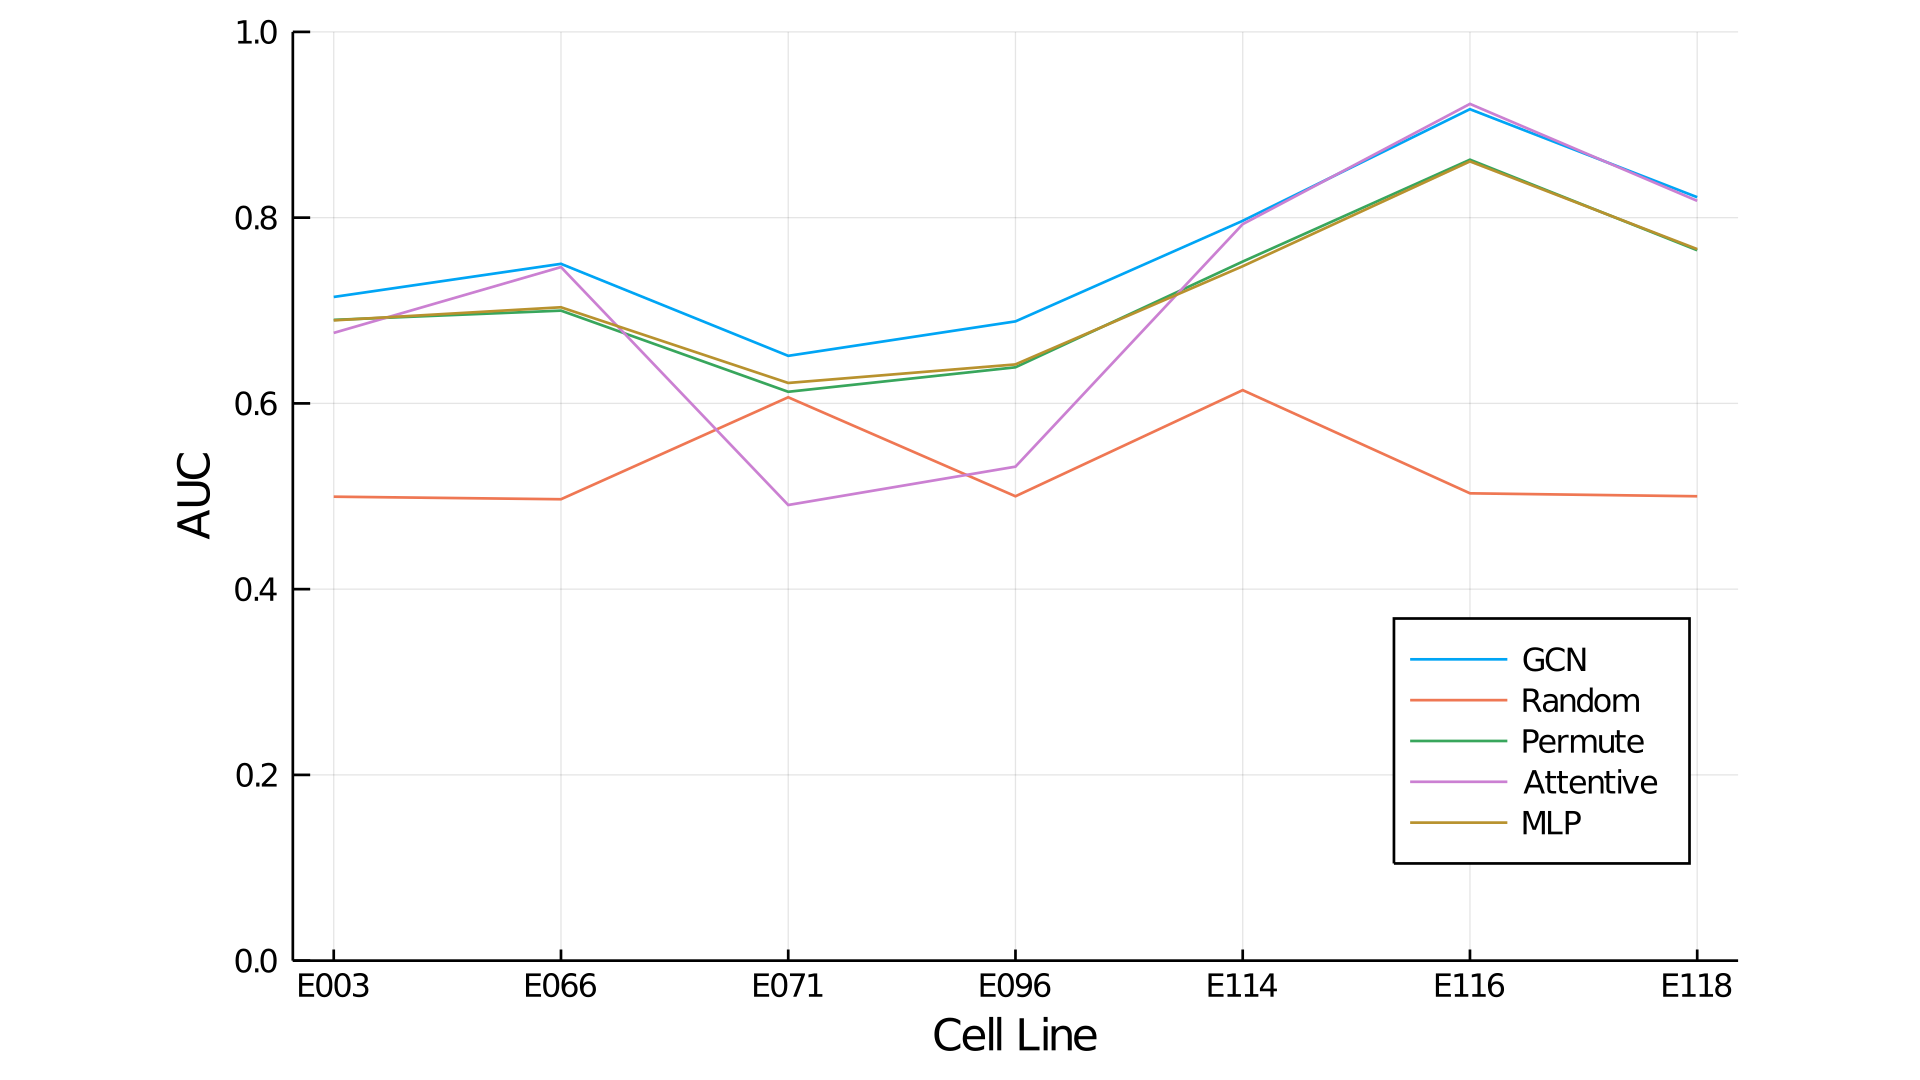
\includegraphics[width=\textwidth]{images/performance.png}
    \caption{AUC Performance Across Cell Lines and Baselines Method}
    \label{figure:Figure1}
\end{figure}
The performance of the model was checked against four baselines across seven different cell lines and is summarized in Table \ref{table:Table1}. \\\\
Quite clearly, the GCN model outperforms almost all of the other baseline methods, including the state of the art AttentiveChrome, across the cell lines. The only cell line where the GCN model was beaten was in the E116 cell line which was high performing across models. It is clear, though, that the GCN model shows great consistency and proves performance gains in lower performing cell lines such as E071. This is encapsulated in the average AUC performance metric across cell lines where the GCN model has a significantly higher average than all other models and in Figure \ref{figure:Figure1}. 
